\documentclass[12pt,a4paper]{article}
\usepackage[left=1in,right=1in,top=1in,bottom=1in]{geometry}
\usepackage[pdftex]{graphicx} 
\usepackage{url} 
\usepackage{afterpage}

\begin{document}
%\renewcommand\bibname{References} 

\begin{titlepage}

\begin{center}

\textup{\small {\bf CS771 Project} \\ Report}\\[0.2in]

\Large \textbf {Separation of foreground frame from background with  high
accuracy in real time}\\[0.5in]
{Department of Computer Science \& Engineering, \\IIT Kanpur }\\[0.2in]

\normalsize Submitted by \\
\begin{table}[h]
\centering
\begin{tabular}{lr} 
Gaurav & 13274 \\
Amit Kumar& 13094 \\
R Sundararajan& 13523\\ \\ 
\end{tabular}
\end{table}

\vspace{.1in}
Under the guidance of\\
{\textbf{Prof. Harish Karnick}}\\[0.2in]

\end{center}
\end{titlepage}
\begin{abstract}
This project is being submitted as the CS771 course project under guidance of Prof Harish Karnick. 
The purpose is to classify the frames as background or foreground with close to perfection.
In this report, we provide the results of the various algorithms we tried to achieve better accuracy.
We first tried standard OpenCV MOG library that resulted in about 92\% accuracy after suitably processing the input frames. Then we shifted to Vibe algorithm which lead to rapid increase in accuracy to about 98\%. Then we implemented the CodeBook Algorithm proposed by Kyungnam Kim and applied certain parameters tweeks to increase accuracy level to 98.37\%.
Observaing the problems in Coodbook we tried to apply edge detection operator on Coodbook results to further enhance the accuracy. Even though the accuracy level improved but the average frame rate fell dramaticaly that lead us to discard the improvement. 
\end{abstract} 
% \section{Motivation}
\section{Algorithms Tried}
\subsection{MOG (Mixture Of Gaussians)}
MOG characterise each pixel by its intensity in the RGB space.The probability of observing a pixel is modelled using a mixture of Gaussian distributions.For each new incoming pixel, the Mahalanobis distance to the distibution is calculated and depending on the threshold, the incoming pixel is classified as background or foreground.In practice, the unmodified output of MOG gives pretty noisy results whereas after blurring the output frame followed by erosion and dilation to we get better contours. 
\subsubsection{Drawbacks}
\begin{itemize}
\item {\bf Foreground Aperture problem :}With backgrounds having fast variations, it becomes difficult to model properly modelled using a few Gaussians.To counter this, if the model is approximated by a large number of Gaussians then slow moving foreground pixels are absorbed into the background resulting in a high false negative rate. 
\item {\bf Shadow problem :}Shadows due to objects outside the frame lead to mis-classification of frames as foreground. And if we tend to remove the shadow Mog tend to remove the entire object on which the shadow falls leading to some foreground frame being classified as back-ground.
\end{itemize} 
\subsection{ViBe}
Vibe is a standard background subtraction algorithm that extracts background features and information from moving frames.
For each pixel values in the past at  its location are stored to maintain adn develop  history model.Now when we need to classify a pixel, we create a sphere of radius R centered a the location. A pixel is classified as background if the number of samples enclosed in the sphere corresponding to its model are greater than a threshold value.Finally, when the pixel is found to be part of the background, its value is propagated into the background model of a neighboring pixel. 
\subsection{Drawbacks}
\begin{itemize}
\item {\bf Stop targets :}If a moving target stops in the field of view for a long time it sends the the target into background thereby misclassifying the frame.
\item {\bf Broken targets :} Splitting the entire target into several pieces because of some parts of target very similar to the background.This leads to quite low bounding box-accuracy  
\end{itemize} 

\subsection{CodeBook Algorithm}
CodeBook algorithm works in two phases, namely learning phase and update phase.Sample background values at each pixel are quantized into codebooks which represent a compressed form of background model much like the bag-of-words representation in text sequences.This helps in capturing background variation due to periodic like motion over a long spam of time with limited memory being used.One of the advantages over other algorithm is that it does not need to be trained on strictly empty frames.Can somewhat handle illumination variations and moving backgrounds but this is better handled using Layered Model Detection.

\section{Drawbacks of CodeBook}
\begin{itemize}
\item {\bf Frame Rate :}CodeBook has quite poor frame rate of 8-9 frames/sec as compared to MOG 20 frames/sec and Vibe 33 frames/sec. 
\item For objects moving far away from the camera, if the contrast between the object and the road is low, it fades into the background.
\item Without layered model detection, the noise rate exceeds the tolerable noise but the static foreground objects are not sent into the background.
\item With layered model detection, the noise is drastically reduced whereas the static foreground objects start being sent into the background albeit very slowly.
\item The parameters have to be separately tuned for different camera angles for different times of the day and the algorithm has to be trained separately for the above different cases.
\end{itemize}

\section{Improving CodeBook}
\subsection{Layered Model Detection(Cache based detection)}
While testing, a cache model (as mentioned in the paper by Kim et al.) is maintained in addition to the original background model generated during training. This helps
backgrounds which were obtained during the detection phase.For this we define an additional cache model and for each incoming pixel at detection time we try to matchin
\begin{itemize}
\item Another way to handle the problem of noisy bounding boxes due to movement of shadows.
\item Results in movement of small stationary foreground pixels into the background thereby drastically reducing the noise.
\end{itemize}

\subsection{Combining codebook's result with an edge detection operator}
The result of the codebook algorithm is combined with an edge detection algorithm (we used Sobel operator).
The main idea is to highlight the boundaries of objects in a scene.This usage of an edge detector will verify if foreground pixels detected by the codebook algorithm b
\begin{itemize}
\item We observed an improvement of (~ 5-7 \%) over the basic codebook algorithm.
\item We obtained an interesting result when working on convex hulls of the contours instead of directly drawing the bounding rectangle of a contour.
\end{itemize}

\begin{figure}[h]
\caption{CodeBook with Sobel edge detector used to draw convex hulls}
\centering
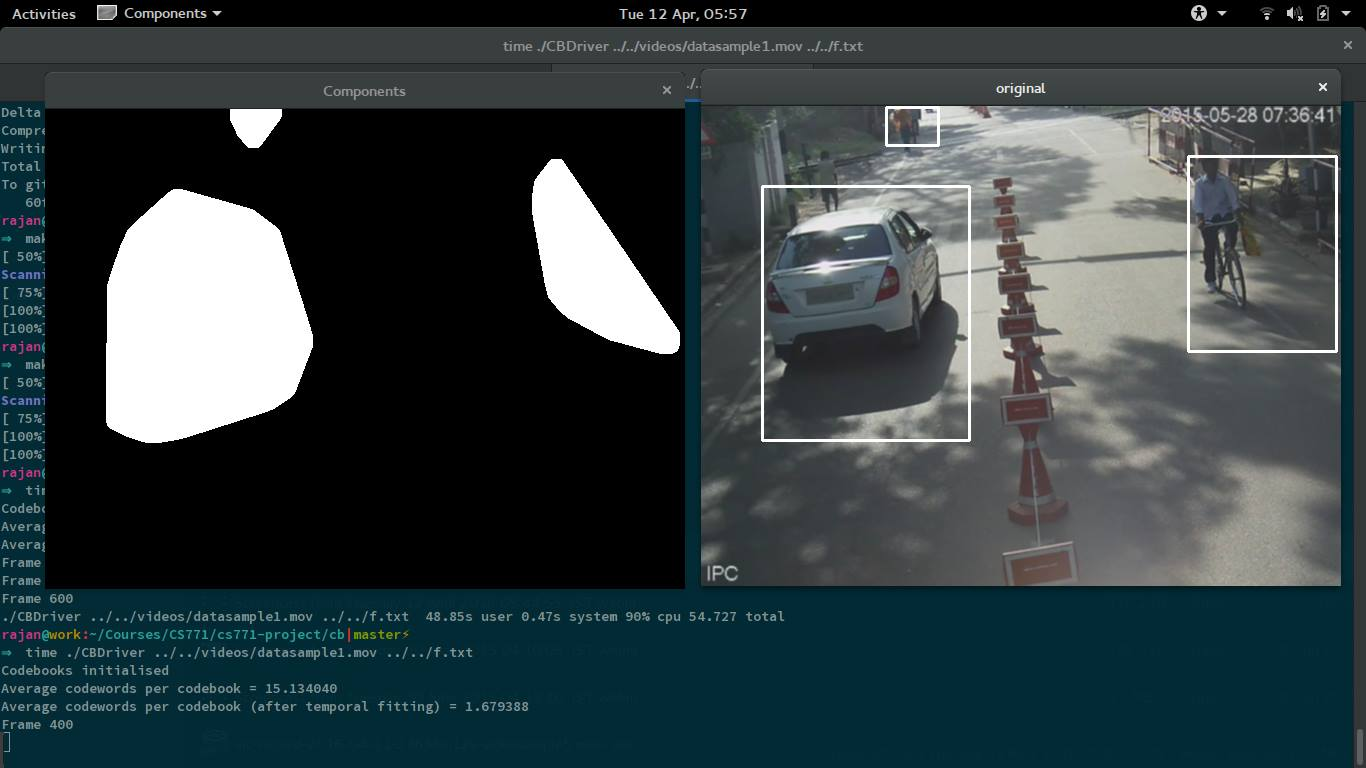
\includegraphics[width=1.0\textwidth]{sobel.png}
\end{figure}

\section{Problems faced and their workarounds made}
\subsection{Implementation level problems}
\begin{itemize}
\item We coded up the CodeBook algorithm on our own
\item \textbf{Problem} : We initially coded up the algorithm in Python but it gave an extremely poor frame rate of 30 frames per minute. This is due to the dynamic typing of python and high overhead associated with the operations on lists and dicitionaries. 
\item \textbf{Solution} : We then switched over to C/C++ which significantly improved the frame rate to 8-9 frames per second. Not too heavy on the size of the codebase (close to 500 lines of code)
\end{itemize}

\subsection{Presence of Noisy contours}
\begin{itemize}
\item \textbf{Problem} : Movement of shadows of trees, illumination changes and shaking of leaves started generating contours of their own.
\item \textbf{Solution}
    \begin{itemize}
    \item All the video is such that no video can have small contours very close to the camera. In fact, these contours are usually due to the movement of the shadows formed by the leaves.
    \item So we increased the minimum area of contours to be drawn close to the camera.
    \item The number of noisy contours detected was drastically reduced.
    \end{itemize}
\end{itemize}

\section{Testing and Results}
\subsection{Steps taken for testing}
\begin{itemize}
\item We annotated frames by adding bounding boxes on our own.
\item We measured accuracy for the \textbf{rectangle (bounding box) overlap} and for overall \textbf{foreground/background binary classification}.
\item For accuracy using rectangle overlap area, we used a test frame set of randomly chosen 35-40 frames from each video sequence.
\item For accuracy of classifying a frame as foreground or background (0-1 accuracy), the test set containing around 700 frames had a 20 \% presence of background frames to ensure their realistic representation in validation.
\end{itemize}

\subsection{Results}
%\begin{table}
\begin{tabular}{l | c | c | c   }   
 & MOG & ViBe & Codebook (edge detection)\\
\hline \hline
Frame Rate& 20 & 33 & 8-9   \\  
Accuracy(B/F) & 92.64 & 98.07 & 98.37 \\
Accuracy(framewise) & 86.39 & 81.07 & 88.13  \\  
Accuracy(overall) & 90.30 & 87.08 & 90.83
\end{tabular}
%\caption{Results}
%\end{table}

\section{Conclusions and Future Scope}
\begin{itemize}
\item We do not have an extremly high accuracy to show for our efforts inspite of trying out quite a lot of variations. The accuracy of our implementation of the CodeBook algorithm is better than those of MOG/ViBe but it is not a significant improvement.
\item The rectangle overlap accuracy cannot be improved to reach a very high percentage such as 99 \% because even a small error in drawing the bounding box of a large foreground object results in a great decrease in the accuracy.
\item But we believe that with better tuning and training, the CodeBook algorithm can achieve greater than 99 \% accuracy for the case of measuring 0-1 accuracy.
\end{itemize}

\section{References}
\begin{itemize}
\item \textbf{ViBe : A universal background subtraction algorithm for video sequences} (Barnich et al.)
\item \textbf{Real time foreground background segmentation using codebook model} (Kim et al.)
\item \textbf{Foreground-Background Segmentation Based on Codebook and Edge Detector} (Mousse et al.)
\end{itemize}

\end{document}
